\section{Results}

\subsection{Stress Validation}
\label{sec:stress-validation}
We first examined whether the VR-TSST successfully induced stress, analysing STAI-S, mean HR, SDNN, and log-transformed HF HRV across the three phases. For each stress-validation measure, we used a one-way repeated-measures ANOVA to test the overall effect of phase, followed by pairwise comparisons between adjacent phases. Pairwise $p$ values were Bonferroni-adjusted across the three phase comparisons for each measure. STAI-S values are reported as scale scores, mean HR in beats per minute (bpm), SDNN in milliseconds (ms), and HF HRV as log-transformed high-frequency spectral power.

STAI-S state scores (~\autoref{fig:hr}-a) showed a significant effect of phase, $F(2,46)=25.77, p<.001$. Self-reported anxiety rose sharply from Baseline ($M=32.38$, $SD=7.83$) to Post-Stress ($M=47.58$, $SD=10.29$; $p<.001$) and then declined at Post-Recovery ($M=35.25$, $SD=11.58$; Post-Stress vs.\ Post-Recovery: $p<.001$), with no significant difference between Baseline and Post-Recovery ($p=.231$). The protocol therefore successfully elevated subjective anxiety during stress induction. The effect was large, $\eta_p^2=.528$; anxiety increased by 15.21 points from Baseline to Post-Stress, 95\% CI $[10.52, 19.89]$.

Mean HR (~\autoref{fig:hr}-b) likewise showed a significant phase effect, $F(2,46)=31.12, p<.001$, increasing from Baseline ($M=88.10$~bpm, $SD=9.03$~bpm) to Stress Induction ($M=92.13$~bpm, $SD=10.62$; $p<.001$) and decreasing at Post-Recovery ($M=83.85$~bpm, $SD=8.41$; Stress Induction vs.\ Post-Recovery: $p<.001$). Baseline and Post-Recovery also differed significantly ($p<.001$), indicating a substantial reduction in physiological arousal after the stress period. The effect was large, $\eta_p^2=.575$; heart rate increased by 4.03~bpm from Baseline to Stress Induction, 95\% CI $[2.06, 6.01]$.

For comparison with prior stress-interaction work, we also examined frequency-domain HF HRV (~\autoref{fig:hr}-c). Log-transformed HF HRV showed a significant effect of phase, $F(2,46)=3.60, p=.035$. The Baseline-to-Stress decrease did not reach significance (Baseline: $M=10.60$, $SD=0.87$; Stress Induction: $M=10.42$, $SD=0.72$; $p=.128$), but HF HRV increased significantly from Stress Induction to Post-Recovery ($M=10.69$, $SD=0.76$; $p=.017$). The effect was moderate, $\eta_p^2=.135$; the Baseline-to-Stress change was $-0.18$, 95\% CI $[-0.42, +0.06]$, and the Stress to Post-Recovery change was $+0.27$, 95\% CI $[+0.05, +0.48]$.

SDNN (~\autoref{fig:hr}-d) showed a significant phase effect, $F(2,46)=8.57, p<.001$, decreasing from Baseline ($M=71.89$~ms, $SD=32.83$) to Stress Induction ($M=56.96$~ms, $SD=19.99$; $p=.005$) and rising again at Post-Recovery ($M=73.31$~ms, $SD=23.47$; $p<.001$). Baseline and Post-Recovery did not differ significantly ($p=.729$). Because lower SDNN reflects reduced HRV and elevated arousal, this pattern provides further evidence that stress induction altered participants' physiological state. The effect was large, $\eta_p^2=.272$; SDNN decreased by 14.93~ms from Baseline to Stress Induction, 95\% CI $[-24.95, -4.91]$, and increased by 16.35~ms from Stress Induction to Post-Recovery, 95\% CI $[+7.69, +25.01]$.

Together, the STAI, HR, and HRV results confirm that the stress-induction protocol elevated both subjective anxiety and physiological arousal. ~\autoref{tab:all-change-summary} summarises the direction and magnitude of percentage change between adjacent phases for ease of comparison.

% \subsection{Validation of Stress Occurrence}

% We first examined whether the VR-TSST successfully induced stress. We analysed STAI-S, mean HR, SDNN, and log-transformed HF HRV across phases. 

% STAI state scores showed a statistically significant effect of phase, $F(2,46)=25.77, p<.001$. Participants reported significantly higher anxiety after stress induction (Baseline: $M=32.38$, $SD=7.83$; Post-Stress: $M=47.58$, $SD=10.29$; Baseline vs.\ Post-Stress: $p<.001$), followed by a significant decrease during Recovery (Recovery: $M=35.25$, $SD=11.58$; Post-Stress vs.\ Recovery: $p<.001$). No significant difference was observed between Baseline and Recovery ($p=.231$). These result shows in ~\autoref{fig:stai} indicate that the protocol successfully increased subjective anxiety during the stress-induction phase.


% Mean HR shows in ~\autoref{fig:hr} also showed a statistically significant effect of phase, $F(2,46)=31.12, p<.001$. Mean HR increased from Baseline ($M=88.10$ bpm, $SD=9.03$) to Stress Induction ($M=92.13$ bpm, $SD=10.62$; Baseline vs.\ Stress Induction: $p<.001$), and significantly decreased during Post-stress Recovery ($M=83.85$ bpm, $SD=8.41$; Stress Induction vs.\ Post-stress Recovery: $p<.001$). Baseline and Recovery also differed significantly ($p<.001$), indicating a substantial reduction in physiological arousal after the stress period.

% We further examined HRV using SDNN. SDNN in ~\autoref{fig:sdnn} showed a significant phase effect, $F(2,42)=8.35, p<.001$. SDNN decreased from Baseline ($M=72.58$ ms, $SD=34.27$) to Stress Induction ($M=57.56$ ms, $SD=21.75$; Baseline vs.\ Stress Induction: $p=.006$), and increased during Post-stress Recovery ($M=73.50$ ms, $SD=22.59$; Stress Induction vs.\ Post-stress Recovery: $p=.001$). Baseline and Recovery did not significantly differ ($p=.819$). Since lower SDNN values indicate reduced HRV and elevated physiological arousal, these results provide further evidence that the stress induction successfully altered participants' physiological state.


% For comparison with prior stress-interaction work, we also examined frequency-domain HF HRV~\ref{fig:hrv_fft}. The repeated-measures ANOVA on log-transformed HF HRV showed a statistically significant effect of phase, $F(2,42)=3.28, p=.047$. Although the decrease from Baseline to Stress Induction did not reach significance (Baseline: $M=10.57$, $SD=0.89$; Stress Induction: $M=10.40$, $SD=0.75$; $p=.122$), HF HRV significantly increased from Stress Induction to Post-stress Recovery (Recovery: $M=10.64$, $SD=0.76$; $p=.017$). 
% Together, the STAI, HR, and HRV results indicate that the stress-induction protocol successfully increased both subjective anxiety and physiological arousal. For ease of comparison across validation measures, ~\autoref{tab:validation-change} summarises the direction and magnitude of percentage changes between adjacent phases.
\begin{figure*}[t]
\centering
\begin{subfigure}[t]{0.24\textwidth}
    \centering
    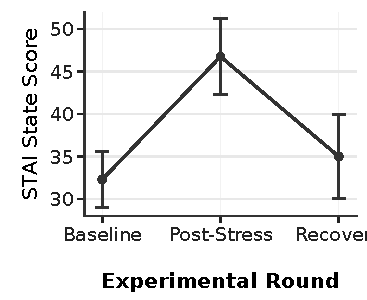
\includegraphics[width=\linewidth]{Figure/stress_stai.pdf}
    \caption{STAI-S}
    \label{fig:stress-stai}
\end{subfigure}\hfill
\begin{subfigure}[t]{0.24\textwidth}
    \centering
    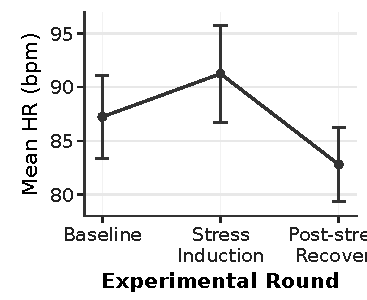
\includegraphics[width=\linewidth]{Figure/stress_hr.pdf}
    \caption{Mean Heart Rate}
    \label{fig:stress-hr}
\end{subfigure}\hfill
\begin{subfigure}[t]{0.24\textwidth}
    \centering
    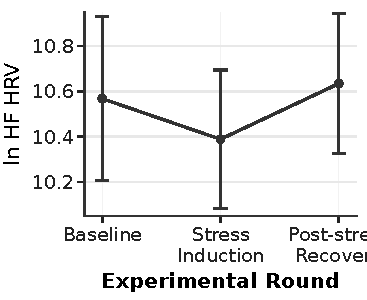
\includegraphics[width=\linewidth]{Figure/stress_hfhrv.pdf}
    \caption{HF HRV}
    \label{fig:stress-hfhrv}
\end{subfigure}\hfill
\begin{subfigure}[t]{0.24\textwidth}
    \centering
    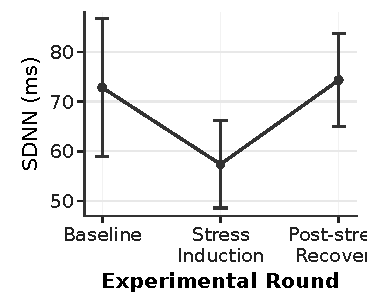
\includegraphics[width=\linewidth]{Figure/stress_sdnn.pdf}
    \caption{SDNN}
    \label{fig:stress-sdnn}
\end{subfigure}

\caption{Validation of stress induction using subjective anxiety and physiological measures. Error bars show 95\% confidence intervals.}
\label{fig:hr}
\end{figure*}

\subsection{Target Acquisition Task}
We next examined target acquisition task performance using mean acquisition time, Fitts' throughput, and spatial offset. One-way repeated-measures ANOVAs showed no significant effect of phase on acquisition time ($F(2,46)=0.10, p=.907$), throughput ($F(2,46)=0.09, p=.912$), or offset ($F(2,46)=0.35, p=.708$), and pairwise comparisons revealed no significant differences between any pair of phases (all $p>.05$). All three effects were negligible in size ($\eta_p^2=.004$, $.004$, and $.015$ for acquisition time, throughput, and offset respectively). Between Baseline and Post-Stress, acquisition time differed by $+17.67$~ms, 95\% CI $[-93.93, +129.26]$; throughput by $-0.02$~bit/s, 95\% CI $[-0.36, +0.33]$; and offset by $+0.05$~cm, 95\% CI $[-0.05, +0.15]$.

Beyond these predefined metrics, we conducted an exploratory analysis of terminal pointing stability, defined as the standard deviation of the finger-to-target-centre offset across the final five samples before successful selection (lower values indicate more stable terminal movements). Mean pre-hit variability (~\autoref{fig:tara}-a) decreased from Baseline ($M=0.341$) to Post-Stress ($M=0.275$) and rose again at Post-Recovery ($M=0.323$). The overall phase effect did not reach significance ($p=.127$), but pairwise comparisons indicated a significant decrease from Baseline to Post-Stress ($p=.025$) and a significant increase from Post-Stress to Post-Recovery ($p=.049$). This suggests that terminal hand movements may have become more stable during the stress phase, even though conventional endpoint measures showed no significant change. ~\autoref{tab:all-change-summary} summarises the phase-wise direction and magnitude of change across target acquisition measures,\autoref{tab:all-change-summary} summarises the observed phase-wise changes in the predefined target acquisition measures and the exploratory pre-hit variability measure.

% \subsubsection{Target Acquisition}

% We then investigated the effect of stress on target acquisition performance using mean target acquisition time, Fitts' throughput, and spatial offset size. A one-way repeated-measures ANOVA showed no statistically significant effect of phase on target acquisition time ($F(2,46)=0.10, p=.907$), throughput ($F(2,46)=0.09, p=.912$), or offset size ($F(2,46)=0.35, p=.708$). Pairwise comparisons also revealed no statistically significant differences between Baseline and Post-Stress or between Post-Stress and Recovery for any of these measures (all $p>.05$). These results indicate that stress induction did not significantly affect target acquisition speed, throughput, or endpoint accuracy in our XR task.

% Beyond the predefined target acquisition metrics, we also conducted an exploratory analysis of terminal pointing stability using the standard deviation of the finger-to-target-center offset during the final five pre-hit samples before successful selection. Lower values indicate more stable hand movements immediately before target acquisition. Mean pre-hit offset variability in ~\autoref{fig:std} decreased from Baseline ($M=0.341$) to Post-Stress ($M=0.275$), and then increased again during Recovery ($M=0.323$). Although the overall phase effect did not reach significance ($p=.127$), pairwise comparisons indicated a significant decrease from Baseline to Post-Stress ($p=.025$) and a significant increase from Post-Stress to Recovery ($p=.049$). This suggests that terminal hand movements may have become more stable during the stress phase, even though conventional endpoint offset measures did not show significant changes. ~\autoref{tab:ta-change} provides a compact summary of the phase-wise direction and magnitude of change across target acquisition measures, highlighting the contrast between stable predefined outcomes and the exploratory terminal stability metric.




\begin{figure}[t]
\centering
\begin{subfigure}[t]{0.48\columnwidth}
    \centering
    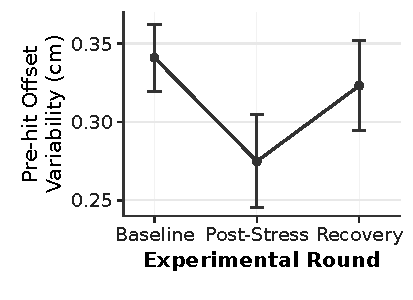
\includegraphics[width=\linewidth]{Figure/prehit_stability.pdf}
    \caption{Exploratory terminal pointing stability}
    \label{fig:prehit-stability}
\end{subfigure}\hfill
\begin{subfigure}[t]{0.48\columnwidth}
    \centering
    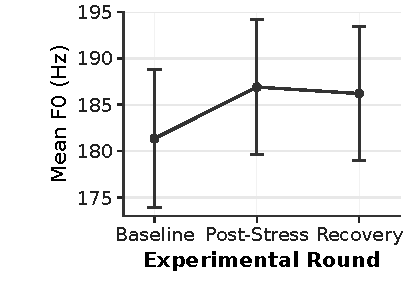
\includegraphics[width=\linewidth]{Figure/reading_mean_f0.pdf}
    \caption{Reading aloud mean F0}
    \label{fig:reading-f0}
\end{subfigure}

\caption{Stress-related changes in target acquisition task and reading aloud task. Error bars show 95\% confidence intervals.}
\label{fig:tara}
\end{figure}
\subsection{Reading Aloud Task}
We then examined reading aloud performance using reading duration, mean fundamental frequency (F0), speech rate, and active speech ratio. A one-way repeated-measures ANOVA showed a significant effect of phase on mean F0 ($F(2,46)=4.26, p=.020$): F0 was higher in Post-Stress ($M=186.91$~Hz, $SD=35.62$) than in Baseline ($M=181.35$~Hz, $SD=36.36$; $p=.020$), but did not differ significantly between Post-Stress and Post-Recovery ($M=186.20$~Hz, $SD=35.38$; $p=.689$). Reading duration, speech rate, and active speech ratio did not show significant effects of phase (all $p>.05$). Mean values are visualised in ~\autoref{fig:tara}-b, and ~\autoref{tab:all-change-summary} summarises the phase-wise percentage changes across vocal measures. The effect on mean F0 was moderate, $\eta_p^2=.156$; F0 rose by 5.55~Hz from Baseline to Post-Stress, 95\% CI $[+0.96, +10.15]$. The remaining vocal measures showed negligible effects: reading duration $F(2,46)=0.27$, $p=.765$, $\eta_p^2=.012$; speech rate $F(2,46)=0.85$, $p=.432$, $\eta_p^2=.036$; active speech ratio $F(2,46)=0.91$, $p=.409$, $\eta_p^2=.038$.

% \subsubsection{Reading Aloud}

% We next examined the effect of stress on read-aloud performance using reading duration, mean fundamental frequency (F0), speech rate, and active speech ratio. The first 3 seconds of each recording were excluded to reduce onset hesitation and recording-start artifacts. A one-way repeated-measures ANOVA showed a statistically significant effect of phase on mean F0 ($F(2,46)=4.26, p=.020$). Pairwise comparisons indicated that mean F0 was significantly higher in the Post-Stress phase ($M=186.91$ Hz, $SD=35.62$) than in Baseline ($M=181.35$ Hz, $SD=36.36$; $p=.020$). However, no statistically significant difference was observed between Post-Stress and Recovery (Recovery: $M=186.20$ Hz, $SD=35.38$; $p=.689$). In contrast, reading duration, speech rate, and active speech ratio did not show statistically significant effects of phase (all $p>.05$). These results suggest that stress induction altered participants' vocal arousal, while leaving coarse speech timing measures relatively stable. The mean values for read-aloud measures are visualised in ~\autoref{fig:ra}, while ~\autoref{tab:ra-change} summarises the phase-wise percentage changes to facilitate comparison across vocal measures.

\subsection{Tower of London Task}
Finally, we examined ToL task performance using first-move latency, move count, total duration, and execution time.
The repeated-measures ANOVA on total duration were not significant ($F(2,46)=2.50, p=.093$). However, pairwise comparisons showed that total duration(~\autoref{fig:tol}-a) was significantly shorter in Post-Stress ($M=36.22$~s, $SD=16.12$) than in Baseline ($M=51.54$~s, $SD=35.86$; $p=.009$), with no significant difference between Post-Stress and Post-Recovery ($M=43.84$~s, $SD=26.00$; $p=.179$). A similar pattern emerged for execution time (~\autoref{fig:tol}-b): the omnibus test was not significant ($F(2,46)=2.26, p=.116$), but execution time was significantly shorter in Post-Stress ($M=20.51$~s, $SD=13.76$) than in Baseline ($M=34.02$~s, $SD=29.02$; $p=.007$), with no significant difference between Post-Stress and Post-Recovery ($p=.348$). First-move latency and move count showed no significant phase effects (all $p>.05$). Both timing effects were small to moderate in size ($\eta_p^2=.098$ for total duration and $.089$ for execution time). Total duration was 15.32~s shorter in Post-Stress than Baseline, 95\% CI $[-26.51, -4.13]$, and execution time 13.52~s shorter, 95\% CI $[-23.00, -4.04]$. The planning measures showed negligible effects: first-move latency $F(2,46)=0.27$, $p=.767$, $\eta_p^2=.011$; move count $F(2,46)=0.80$, $p=.456$, $\eta_p^2=.034$.

These results indicate that stress induction did not broadly improve ToL planning performance but was associated with faster task execution following stress. This reduction in execution time should be interpreted cautiously, as it may reflect more hurried or urgent execution rather than a genuine enhancement of planning ability. ~\autoref{tab:all-change-summary} summarises the direction and relative magnitude of phase-wise changes across ToL measures, showing that the clearest shifts occurred in total duration and execution time rather than in planning-specific measures.
% \subsubsection{Tower of London}

% We then investigated the effect of stress on Tower of London (ToL) performance using first-move latency, move count, total duration and execution time. Execution time was computed as total task duration minus first-move latency, capturing the time spent executing moves after the initial planning period.

% A one-way repeated-measures ANOVA did not show a statistically significant effect of phase on total duration ($F(2,46)=2.28, p=.114$)~\ref{fig:tol_dur}. However, pairwise comparisons indicated that total duration was significantly shorter in the Post-Stress phase ($M=36.22$ s, $SD=16.12$) than in Baseline ($M=50.87$ s, $SD=36.30$; $p=.013$). No statistically significant difference was observed between Post-Stress and Recovery (Recovery: $M=44.51$ s, $SD=25.58$; $p=.147$).


\begin{figure}[t]
\centering
\begin{subfigure}[t]{0.48\columnwidth}
    \centering
    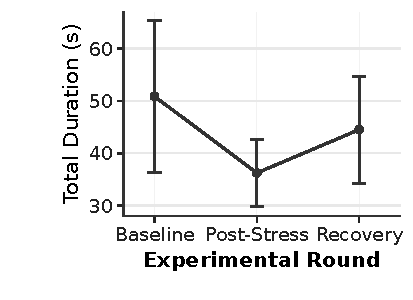
\includegraphics[width=\linewidth]{Figure/tol_total_duration.pdf}
    \caption{Total duration}
    \label{fig:tol-duration}
\end{subfigure}
\begin{subfigure}[t]{0.48\columnwidth}
    \centering
    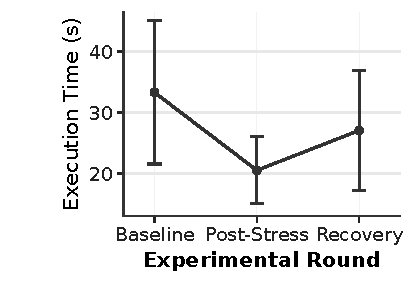
\includegraphics[width=\linewidth]{Figure/tol_execution_time.pdf}
    \caption{Execution time}
    \label{fig:tol-execution}
\end{subfigure}\hfill


\caption{Tower of London timing measures across experimental phases. Error bars show 95\% confidence intervals.}
\label{fig:tol}
\end{figure}
% Similarly, a one-way repeated-measures ANOVA did not show a statistically significant effect of phase on execution time ($F(2,46)=1.98, p=.149$)~\ref{fig:tol_exe}. Nevertheless, pairwise comparisons showed that execution time was significantly shorter in the Post-Stress phase ($M=20.51$ s, $SD=13.76$) than in Baseline ($M=33.29$ s, $SD=29.38$; $p=.010$). No statistically significant difference was found between Post-Stress and Recovery ($p=.295$).

% In contrast, first-move latency and move count did not show statistically significant effects of phase (all $p>.05$). Taken together, these results indicate that stress induction did not broadly improve ToL planning performance, but was associated with faster task execution following stress induction. This reduction in execution time should be interpreted cautiously, as it may reflect faster or more urgent task execution rather than a broad enhancement of planning ability. ~\autoref{tab:tol-change} summarises the direction and relative magnitude of phase-wise changes across Tower of London measures, showing that the clearest shifts were observed in total duration and execution time rather than in planning-specific measures.


\subsection{Participant Feedback}
Post-study interviews suggested that participants did not experience the stress induction in a uniform way. Seven participants reported feeling more focused during the post-stress tasks, whereas three reported little or no noticeable change and four found the change difficult to describe. Participants also differed in which part of the VR-TSST they found most stressful: thirteen identified the mental arithmetic phase as more stressful than the speech phase, while three reported that the speech task felt less stressful because the audience consisted of virtual characters rather than real people. However, this pattern was not universal; one participant reported feeling ashamed during the speech task, and two participants noted that not being able to see their hands during the induction increased their tension in VR.
Several comments were also consistent with the behavioural results. Three participants explicitly stated that, after stress induction, they wanted to complete the subsequent tasks more quickly, which aligns with the shorter execution time observed in the Tower of London task. At the same time, one participant reported feeling calmer after the induction and found the later tasks easier, highlighting individual differences in post-stress responses. Overall, the interviews suggest that the VR-TSST elicited a mixture of heightened pressure, narrowed attention, altered embodiment, and task-focused urgency rather than a single uniform subjective response.

\begin{table}[t]
\centering
\large
\caption{Summary of stress-related changes across validation and task measures. Colored arrows indicate statistically significant pairwise differences ($p < .05$), whereas black arrows denote descriptive but non-significant changes. * denotes an exploratory metric.}
\label{tab:all-change-summary}
\normalsize
\resizebox{\columnwidth}{!}{
\begin{tabular}{lcc}
\toprule
\textbf{Measure} & \textbf{Baseline $\rightarrow$ Post-Stress} & \textbf{Post-Stress $\rightarrow$ Post-Recovery} \\
\midrule

\multicolumn{3}{l}{\textbf{Stress validation}} \\
\quad STAI-S
& \textcolor{orange}{\(\uparrow\) 46.9\%}
& \textcolor{blue}{\(\downarrow\) 25.9\%} \\
\quad Mean HR
& \textcolor{orange}{\(\uparrow\) 4.6\%}
& \textcolor{blue}{\(\downarrow\) 9.0\%} \\
\quad SDNN
& \textcolor{blue}{\(\downarrow\) 20.8\%}
& \textcolor{orange}{\(\uparrow\) 28.7\%} \\
\quad ln HF HRV
& \textcolor{black}{\(\downarrow\) 1.7\%}
& \textcolor{orange}{\(\uparrow\) 2.6\%} \\

\midrule
\multicolumn{3}{l}{\textbf{Target acquisition}} \\
\quad MT
& \textcolor{black}{\(\uparrow\) 2.0\%}
& \textcolor{black}{\(\downarrow\) 2.0\%} \\
\quad Offset
& \textcolor{black}{\(\uparrow\) 2.5\%}
& \textcolor{black}{\(\downarrow\) 0.5\%} \\
\quad TP
& \textcolor{black}{\(\downarrow\) 0.5\%}
& \textcolor{black}{\(\downarrow\) 1.9\%} \\
\quad Pre-hit Stability*
& \textcolor{blue}{\(\downarrow\) 19.4\%}
& \textcolor{orange}{\(\uparrow\) 17.5\%} \\

\midrule
\multicolumn{3}{l}{\textbf{Reading aloud}} \\
\quad Mean F0
& \textcolor{orange}{\(\uparrow\) 3.1\%}
& \textcolor{black}{\(\downarrow\) 0.4\%} \\
\quad Speech Rate
& \textcolor{black}{\(\uparrow\) 1.0\%}
& \textcolor{black}{\(\downarrow\) 3.6\%} \\
\quad Reading Duration
& \textcolor{black}{\(\uparrow\) 1.5\%}
& \textcolor{black}{\(\downarrow\) 2.3\%} \\
\quad Active Speech Ratio
& \textcolor{black}{\(\downarrow\) 0.6\%}
& \textcolor{black}{\(\downarrow\) 3.7\%} \\

\midrule
\multicolumn{3}{l}{\textbf{Tower of London}} \\
\quad First-Move Latency
& \textcolor{black}{\(\downarrow\) 10.6\%}
& \textcolor{black}{\(\uparrow\) 11.1\%} \\
\quad Move Count
& \textcolor{black}{\(\downarrow\) 6.2\%}
& \textcolor{black}{\(\uparrow\) 15.3\%} \\
\quad Total Duration
& \textcolor{blue}{\(\downarrow\) 29.7\%}
& \textcolor{black}{\(\uparrow\) 22.9\%} \\
\quad Execution Time
& \textcolor{blue}{\(\downarrow\) 39.7\%}
& \textcolor{black}{\(\uparrow\) 31.8\%} \\

\bottomrule
\end{tabular}
}
\end{table}